\section{Cycle Definitions}

Building on the definitions and properties of lists, we now define Cycles.

A Cycle is an unbounded list that repeats a finite sequence of elements from a
bounded list. In this study, we restrict our universe of values $\mathbb{S}$ to
be the set of non-negative integers, i.e., $\mathbb{S}=\mathbb{N}_0$.

\begin{itemize}
  \item Recursive: values at $i$ where $i<n$ come from the base list,
    otherwise recurse on $i-n$ --- the definitional spec.
  \item Modulo: values come directly from the base list at position
    $i\bmod n$ --- efficient access.
  \item Memory: wraps \texttt{ModCycle}, adds classification tracking via
    \texttt{checkMod(d)} --- remembers which divisors produce all-zero,
    some-zero, or none-zero residue patterns.
\end{itemize}

\begin{figure}[htbp]
  \centering
  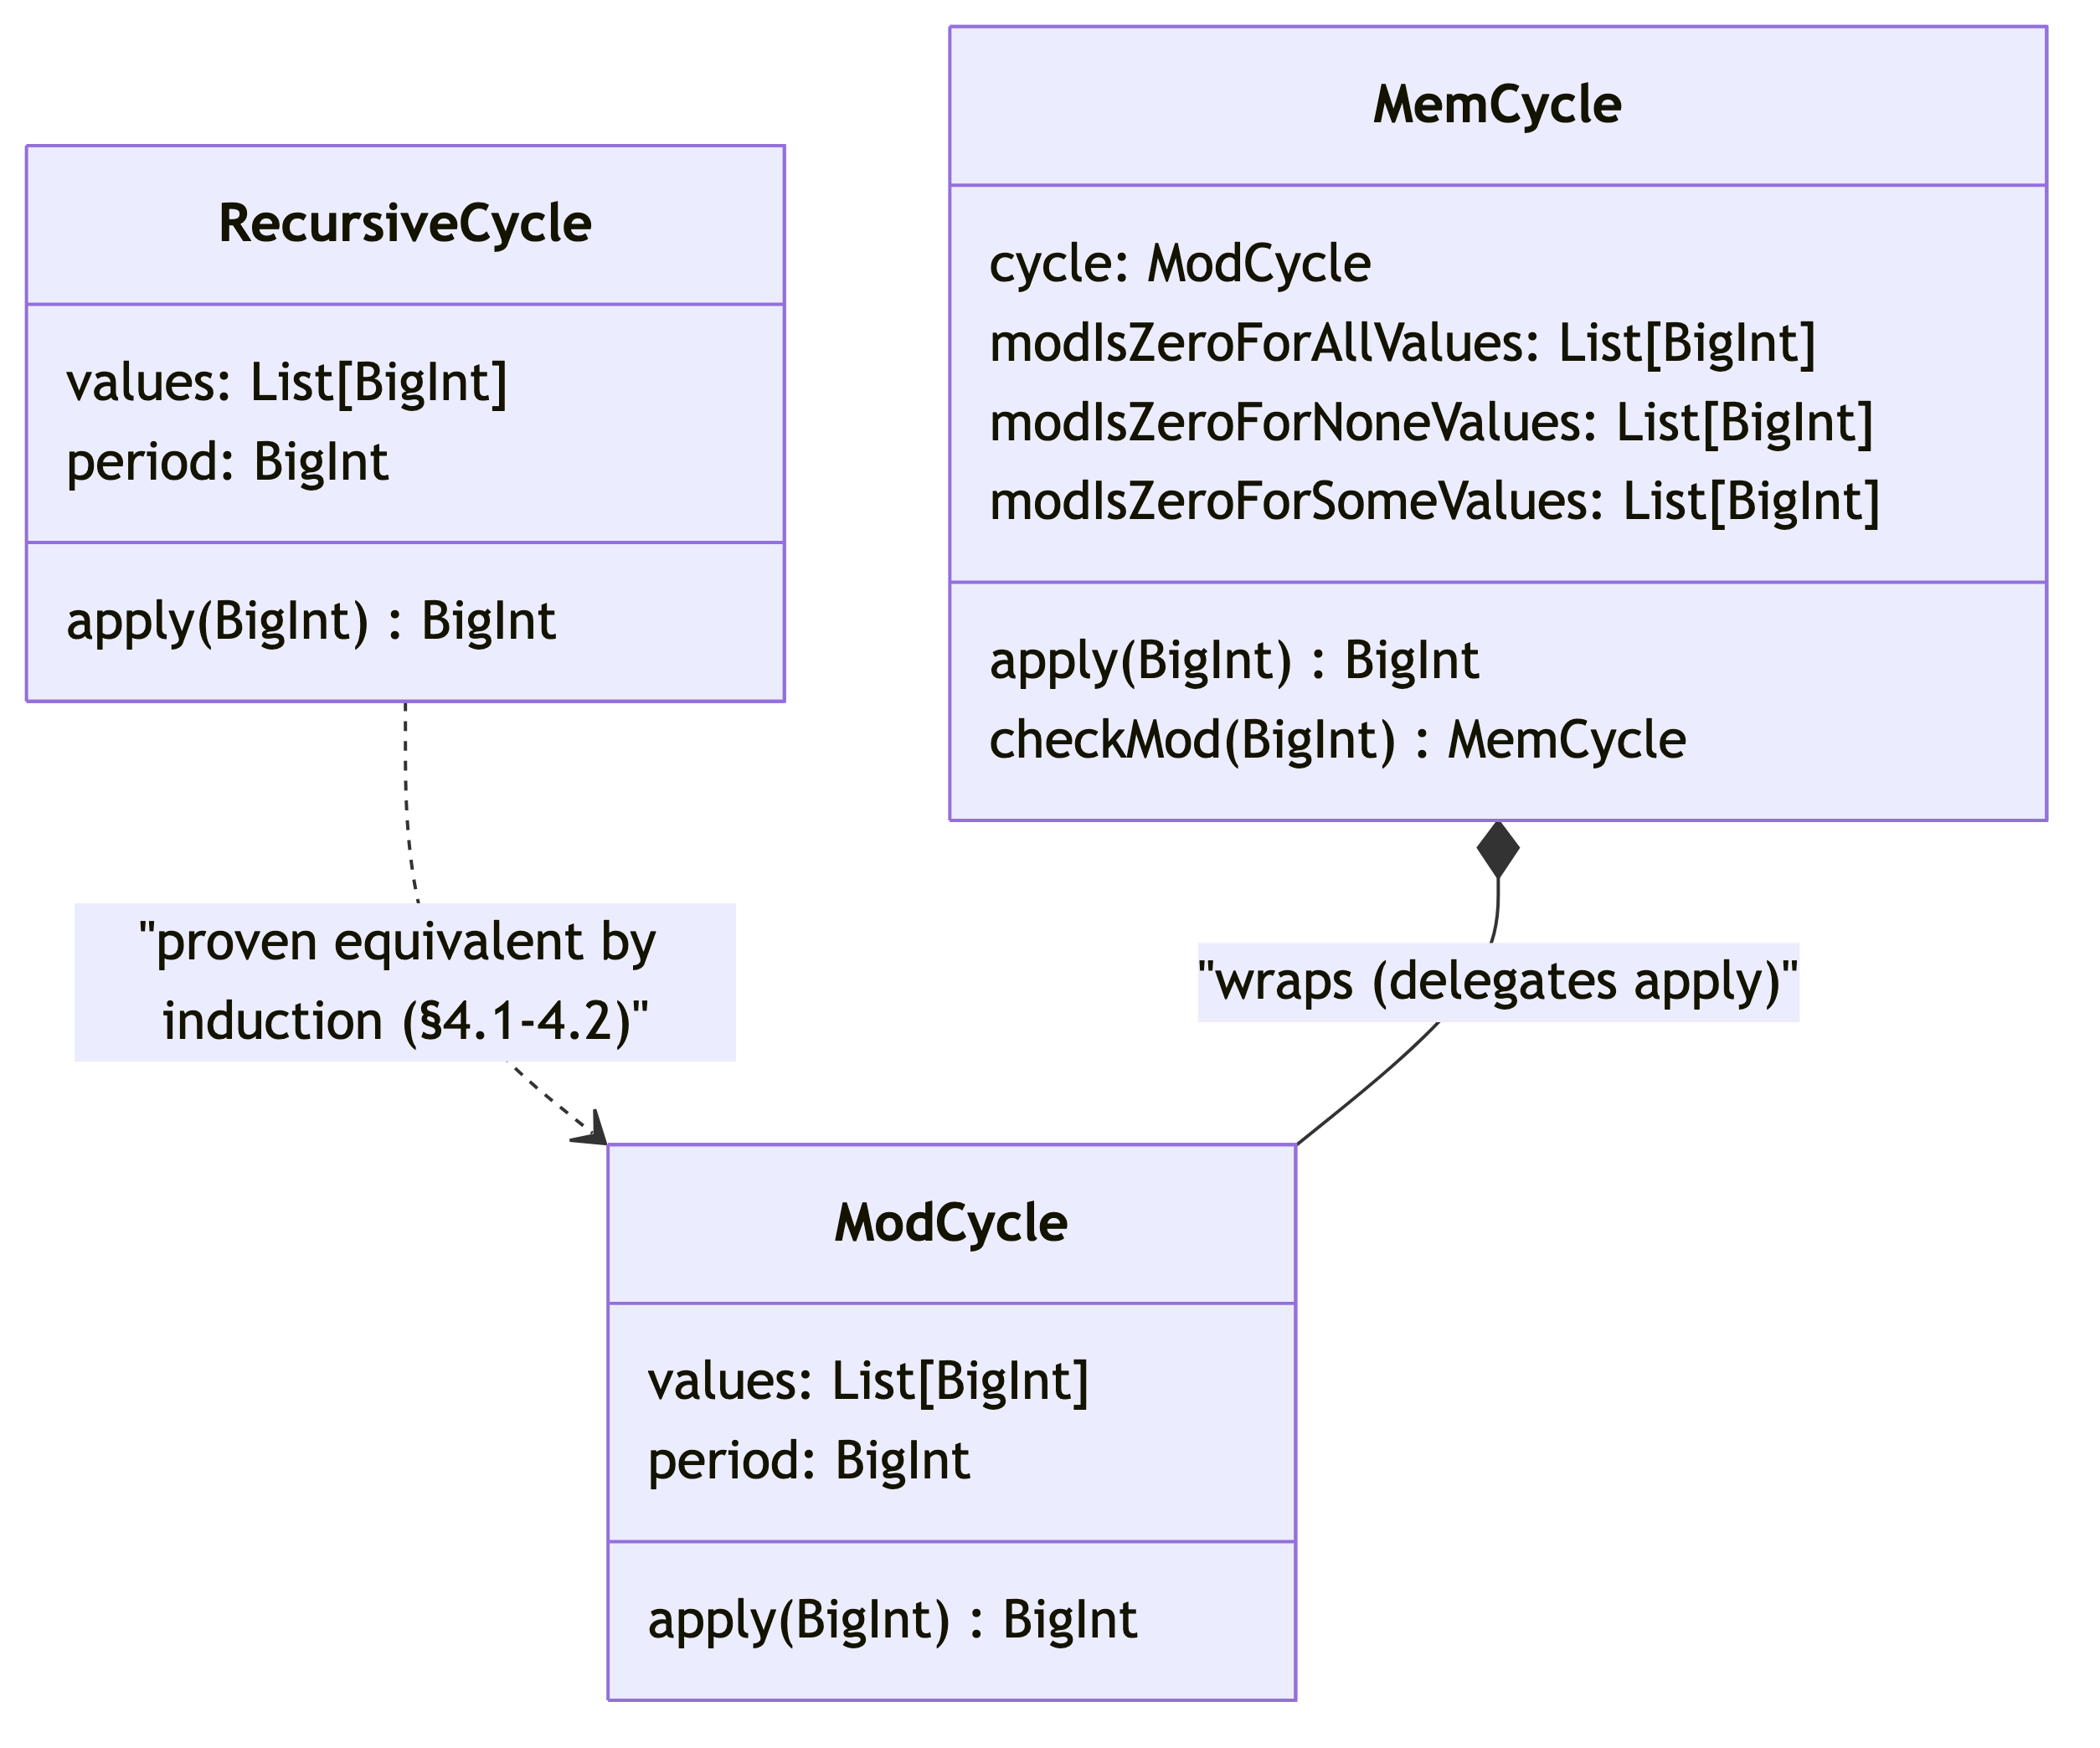
\includegraphics[width=0.92\linewidth]{figures/cycle-classes.png}
\end{figure}

\subsection{Recursive Cycle}

\begin{equation*}
\begin{aligned}
\forall\, L\in\mathbb{L},\quad \forall\, v&\in\mathbb{N}_0,
  \quad \forall\, i\in\mathbb{N}_0 \\
L &:= [v_0,v_1,\dots,v_{n-1}]\in\mathbb{N}_0^n \\
n &= |L| \\
\operatorname{RecCycle}_i &:=
\begin{cases}
L_i & \text{if } i<n \\
\operatorname{RecCycle}_{i-n} & \text{if } i\geq n
\end{cases},\quad |L|>0 \\
&\therefore \\
\operatorname{RecCycle}
  &= [v_0,v_1,\dots,v_{n-1},v_0,v_1,\dots] \\
\operatorname{Cycle}_i &:= \operatorname{RecCycle}_i
\end{aligned}
\end{equation*}

We take this recursive unrolling as the formal ground truth for the informal
picture of ``the infinite periodic sequence'' used throughout this article:
from here on, \texttt{Cycle} means \texttt{RecCycle}. That is a naming choice,
not a theorem --- the recursion peels off one copy of the base list per step,
which is exactly what the periodic sequence means. What still needs proof is
whether the modulo-based definition below computes the same values; that
equivalence is proved in Section~4.

The recursive cycle is defined at
\href{https://github.com/thiagomata/prime-numbers/blob/cycle-article-v1.0.0/src/main/scala/v1/chapter4/cycle/recursive/RecursiveCycle.scala}{\texttt{RecursiveCycle}}:

\begin{lstlisting}[style=scala]
case class RecursiveCycle(values: List[BigInt]) {
  require(values.nonEmpty)
  require(CycleUtils.checkPositiveOrZero(values))

  def period: BigInt = values.size

  def apply(position: BigInt): BigInt = {
    decreases(position)
    require(position >= 0)

    if (position < period) {
      values(position)
    } else {
      apply(position - values.size)
    }
  }
}
\end{lstlisting}

\subsection{Modulo Cycle}

A Cycle can also be defined using modulo arithmetic, which is a common approach
in computer science to handle cyclic structures.

\begin{equation*}
\begin{aligned}
\forall\, L\in\mathbb{L},\quad \forall\, v&\in\mathbb{N}_0,
  \quad \forall\, i\in\mathbb{N}_0 \\
L &:= [v_0,v_1,\dots,v_{n-1}]\in\mathbb{N}_0^n \\
n &= |L| \\
\operatorname{ModCycle}_i &= L[i\operatorname{mod}n],\quad |L|>0 \\
&\therefore \\
\operatorname{ModCycle}
  &= [v_0,v_1,\dots,v_{n-1},v_0,v_1,\dots]
\end{aligned}
\end{equation*}

This unrolls informally to the same picture, but nothing so far shows that
\texttt{ModCycle} and \texttt{RecCycle} --- which Subsection~3.1 took as the
meaning of \texttt{Cycle} --- agree at every index. One recurses by repeated
subtraction, the other computes a single remainder, and it is not obvious a
priori that the two produce the same sequence. Section~4 proves they do, which
is what lets \texttt{ModCycle} stand in for \texttt{Cycle} as well.

The modulo cycle is defined at
\href{https://github.com/thiagomata/prime-numbers/blob/cycle-article-v1.0.0/src/main/scala/v1/chapter4/cycle/mod/ModCycle.scala}{\texttt{ModCycle}}:

\begin{lstlisting}[style=scala]
case class ModCycle(values: List[BigInt]) {
  require(CycleUtils.checkPositiveOrZero(values))
  require(values.nonEmpty)

  def apply(position: BigInt): BigInt = {
    require(position >= 0)
    val index = Calc.mod(position, values.size)
    assert(index >= 0)
    assert(index < values.size)
    values(index)
  }

  def period: BigInt = values.size

  def sum(): BigInt = ListUtils.sum(values)
}
\end{lstlisting}

\subsection{Memory Cycle}

The third representation, \texttt{MemCycle}, wraps a \texttt{ModCycle} and
adds classification state: three lists tracking which divisors produce
all-zero, some-zero, or none-zero residue patterns across the cycle's values.

Like ModCycle, positional lookup uses modular indexing; value access delegates
directly to the wrapped ModCycle. Positional equivalence between the two is
immediate by construction: \texttt{MemCycle.apply(position)} calls the wrapped
\texttt{cycle(position)}, and \texttt{MemCycle(values)} constructs that wrapped
cycle as \texttt{ModCycle(values)}.

\begin{equation*}
\begin{aligned}
\operatorname{MemCycle}(L)_i
  &= \operatorname{ModCycle}(L)_i
  && \text{[By MemCycle.apply delegating to its wrapped ModCycle]}
\end{aligned}
\end{equation*}

The bounded bridge
\href{https://github.com/thiagomata/prime-numbers/blob/cycle-article-v1.0.0/src/main/scala/v1/chapter4/cycle/properties/CycleProperties.scala}{\texttt{CycleProperties::assertModCycleEqualsMemCycle}}
verifies the same lookup equality over one physical period for a
\texttt{ModCycle} and a \texttt{MemCycle} sharing the same values and period.

\texttt{MemCycle(L)} returns the same values as \texttt{ModCycle(L)} by
definition: it stores \texttt{ModCycle(L)} and delegates every lookup to it.
Section~4 proves the remaining piece --- that \texttt{RecursiveCycle(L)} and
\texttt{ModCycle(L)} also agree at every position --- after which the full
three-way equality chain used throughout the article is assembled at the close
of that section.

The cycle is immutable. Calling \texttt{checkMod(d)} returns a \emph{new}
\texttt{MemCycle} with \texttt{d} added to the appropriate classification
list. The original is unchanged. Values are never modified; classification is
metadata accumulated across calls.

\begin{lstlisting}[style=scala]
case class MemCycle private (
  cycle: ModCycle,
  modIsZeroForAllValues: List[BigInt] = List.empty,
  modIsZeroForNoneValues: List[BigInt] = List.empty,
  modIsZeroForSomeValues: List[BigInt] = List.empty,
) {
  def apply(position: BigInt): BigInt = cycle(position)
  def values: List[BigInt] = cycle.values
  def period: BigInt = cycle.period
  def checkMod(dividend: BigInt): MemCycle = { /* returns new MemCycle */ }
}
\end{lstlisting}

The memory cycle is defined at
\href{https://github.com/thiagomata/prime-numbers/blob/cycle-article-v1.0.0/src/main/scala/v1/chapter4/cycle/memory/MemCycle.scala}{\texttt{MemCycle}}.
Classification lemmas are verified in
\href{https://github.com/thiagomata/prime-numbers/blob/cycle-article-v1.0.0/src/main/scala/v1/chapter4/cycle/memory/properties/CycleCheckMod.scala}{\texttt{CycleCheckMod}}.
